\documentclass[a4paper, 14pt]{extarticle}

% Поля
%--------------------------------------
\usepackage{geometry}
\geometry{a4paper,tmargin=2cm,bmargin=2cm,lmargin=3cm,rmargin=1cm}
%--------------------------------------


%Russian-specific packages
%--------------------------------------
\usepackage[T2A]{fontenc}
\usepackage[utf8]{inputenc} 
\usepackage[english, main=russian]{babel}
%--------------------------------------

\usepackage{textcomp}

% Красная строка
%--------------------------------------
\usepackage{indentfirst}               
%--------------------------------------             


%Graphics
%--------------------------------------
\usepackage{graphicx}
\graphicspath{ {./images/} }
\usepackage{wrapfig}
%--------------------------------------

% Полуторный интервал
%--------------------------------------
\linespread{1.3}                    
%--------------------------------------

%Выравнивание и переносы
%--------------------------------------
% Избавляемся от переполнений
\sloppy
% Запрещаем разрыв страницы после первой строки абзаца
\clubpenalty=10000
% Запрещаем разрыв страницы после последней строки абзаца
\widowpenalty=10000
%--------------------------------------

%Списки
\usepackage{enumitem}

%Подписи
\usepackage{caption} 

%Гиперссылки
\usepackage{hyperref}

\hypersetup {
	unicode=true
}

%Рисунки
%--------------------------------------
\DeclareCaptionLabelSeparator*{emdash}{~--- }
\captionsetup[figure]{labelsep=emdash,font=onehalfspacing,position=bottom}
%--------------------------------------

\usepackage{tempora}
\usepackage{amsmath}
\usepackage{color}
\usepackage{listings}
\lstset{
  belowcaptionskip=1\baselineskip,
  breaklines=true,
  frame=L,
  xleftmargin=\parindent,
  language=Python,
  showstringspaces=false,
  basicstyle=\footnotesize\ttfamily,
  keywordstyle=\bfseries\color{blue},
  commentstyle=\itshape\color{purple},
  identifierstyle=\color{black},
  stringstyle=\color{red},
}

%--------------------------------------
%			НАЧАЛО ДОКУМЕНТА
%--------------------------------------

\begin{document}

%--------------------------------------
%			ТИТУЛЬНЫЙ ЛИСТ
%--------------------------------------
\begin{titlepage}
\thispagestyle{empty}
\newpage


%Шапка титульного листа
%--------------------------------------
\vspace*{-60pt}
\hspace{-65pt}
\begin{minipage}{0.3\textwidth}
\hspace*{-20pt}\centering

\includegraphics[width=\textwidth]{emblem}
\end{minipage}
\begin{minipage}{0.67\textwidth}\small \textbf{
\vspace*{-0.7ex}
\hspace*{-6pt}\centerline{Министерство науки и высшего образования Российской Федерации}
\vspace*{-0.7ex}
\centerline{Федеральное государственное бюджетное образовательное учреждение }
\vspace*{-0.7ex}
\centerline{высшего образования}
\vspace*{-0.7ex}
\centerline{<<Московский государственный технический университет}
\vspace*{-0.7ex}
\centerline{имени Н.Э. Баумана}
\vspace*{-0.7ex}
\centerline{(национальный исследовательский университет)>>}
\vspace*{-0.7ex}
\centerline{(МГТУ им. Н.Э. Баумана)}}
\end{minipage}
%--------------------------------------

%Полосы
%--------------------------------------
\vspace{-25pt}
\hspace{-35pt}\rule{\textwidth}{2.3pt}

\vspace*{-20.3pt}
\hspace{-35pt}\rule{\textwidth}{0.4pt}
%--------------------------------------

\vspace{1.5ex}
\hspace{-35pt} \noindent \small ФАКУЛЬТЕТ\hspace{80pt} <<Информатика и системы управления>>

\vspace*{-16pt}
\hspace{47pt}\rule{0.83\textwidth}{0.4pt}

\vspace{0.5ex}
\hspace{-35pt} \noindent \small КАФЕДРА\hspace{50pt} <<Прикладная Математика и информатика>>

\vspace*{-16pt}
\hspace{30pt}\rule{0.866\textwidth}{0.4pt}
  
\vspace{11em}

\begin{center}
\Large {\bf "Летучка" 1} \\ 
\large {\bf по курсу <<Языки и методы программирования>>} \\ 
\large <<Реализация простейшего класса по вариантам>>
\end{center}\normalsize

\vspace{8em}


\begin{flushright}
  {Студент группы ИУ9-21Б Хромов М.А.\hspace*{15pt} \\
  \vspace{2ex}
  Преподаватель Посевин Д. П.\hspace*{15pt}}
\end{flushright}

\bigskip

\vfill
 

\begin{center}
\textsl{Москва 2025}
\end{center}
\end{titlepage}
%--------------------------------------
%		КОНЕЦ ТИТУЛЬНОГО ЛИСТА
%--------------------------------------

\renewcommand{\ttdefault}{pcr}

\setlength{\tabcolsep}{3pt}
\newpage


 

\section{Задание}\label{Sect::task}
\par
Необходимо реализовать класс с одним полем и методом предоставлящим доступ к
этому пол. Начальное значение поля класса задается в конструкторе в функции main,
необходимо определить экземпляр класса, вывести дефолтное значение поля, передать
инициализированному объекту сообщение об изменении состояния этого объекта и вывести
выполненное изменение на экран. Принцип инкапсуляции должен соблдаться
Программа должна быть запущена на одном из серверов, и сохранена до момента
проверки преподавателем в том же месте, где была создана и отлажена. Факт того, что она
выполнена должен быть подтвержден скриншотом и скриншотом вывода команды ls -lsa.
При запуске программа должна выводить фамили, имя и группу студента.
\section{Индивидуальный вариант}\label{Sect::task}
\par
Класс автомобиль с состоянием заведен или не заведен. При инициализации он не заведен.
\section {Практическая реализация}
Исходный код программы представлен в листинге
\begin{figure}[!htb]
\begin{lstlisting}[language={},caption={реализация},label={lst:code1}]
public class Main {
    public static void main(String[] args) {

        System.out.println("Фамилия: Хромов");
        System.out.println("Имя: Матвей");
        System.out.println("Группа: ИУ9-21Б");


        Car myCar = new Car(false);


        System.out.println("\nСостояние двигателя при создании: " +
                (myCar.isEngineOn() ? "Заведен" : "Не заведен"));


        myCar.setEngineOn(true);


        System.out.println("Новое состояние двигателя: " +
                (myCar.isEngineOn() ? "Заведен" : "Не заведен"));
    }
}

class Car {
    private boolean isEngineOn;


    public Car(boolean isEngineOn) {
        this.isEngineOn = isEngineOn;
    }


    public boolean isEngineOn() {
        return isEngineOn;
    }


    public void setEngineOn(boolean engineStatus) {
        this.isEngineOn = engineStatus;
    }
}
\end{lstlisting}
\end{figure}
\clearpage
\newpage

\section{Реализация}

\begin{center}
    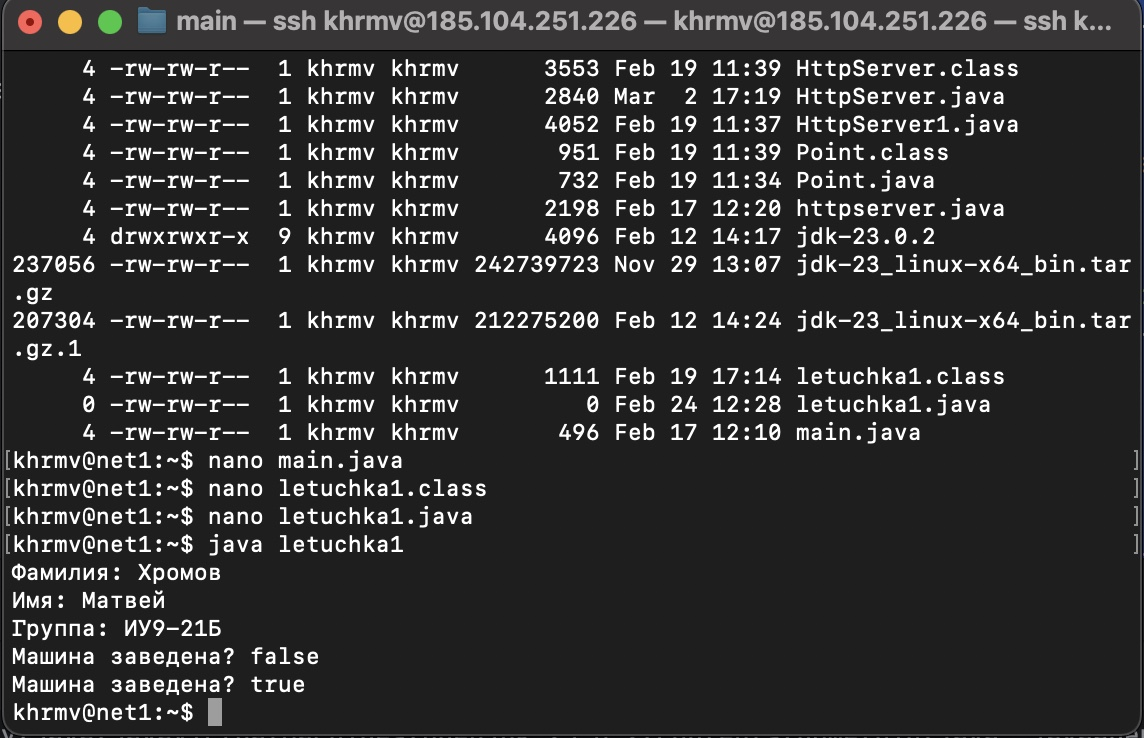
\includegraphics[width=0.8\textwidth]{фото16.jpeg}
    \captionof{figure}{терминал}
\end{center}
\newpage
\section{Вывод}
В ходе работы был реализован класс Car с инкапсулированным полем isEngineOn, управляемым через геттер и сеттер. Начальное состояние двигателя (не заведен) задавалось в конструкторе, после чего программа выводила его, изменяла состояние на "заведен" и отображала результат. Принципы инкапсуляции соблюдены: доступ к полю осуществляется только через методы.

\end{document}